\documentclass{article}
\usepackage{amsmath,amsthm,amssymb,amsfonts}
\usepackage{setspace,enumitem}
\usepackage{graphicx}
\usepackage{hyperref}
\usepackage{natbib}
\usepackage{lscape}
\usepackage{afterpage}
\usepackage{xcolor}
\usepackage{etoolbox}
\usepackage{booktabs}
\usepackage{pdfpages}
\usepackage{multicol}
\usepackage{geometry}
\usepackage{accents}
\usepackage{bbm}
\usepackage{verbatim}
\usepackage{lscape}

\setlength{\parindent}{0cm}
\geometry{margin = 1in}

\newcommand{\R}{\mathbb{R}}
\newcommand{\ubar}[1]{\underaccent{\bar}{#1}}
\newcommand{\Int}{\text{Int}}
\newcommand{\xbf}{\mathbf{x}}
\newcommand{\Abf}{\mathbf{A}}
\newcommand{\Bbf}{\mathbf{B}}
\newcommand{\Gbf}{\mathbf{G}}
\newcommand{\bbf}{\mathbf{b}}
\newcommand{\one}{\mathbbm{1}}

\newtoggle{extended}
\settoggle{extended}{false}

\title{ECON 717A: Problem Set 1}
\author{Alex von Hafften }

\begin{document}

\maketitle

\section{Write-Up}

\subsection*{Problem 1 - Dropping Miss Values}

I drop observations with missing values for \texttt{HH\_Income} as well as observations with indicators \texttt{miss\_Client\_Age}, \texttt{miss\_Client\_Married}, and \texttt{miss\_Client\_Education} equaling one.  This filtering drops 65 observations.

\subsection*{Problem 2 - LPM}

I estimate a linear probability model with homoskedastic standard errors of \texttt{taken\_new} on \texttt{Client\_Age}, \texttt{Client\_Married}, \texttt{Client\_Education}, \texttt{HH\_Size}, \texttt{HH\_Income}, \texttt{muslim}, \texttt{Hindu\_SC\_Kat}, and \texttt{Treated}.

\bigskip

\begin{center}
\begin{tabular}{lc} \hline
 & (1) \\
VARIABLES & taken\_new \\ \hline
 &  \\
Client\_Age & -2.83e-05 \\
 & (0.00216) \\
Client\_Married & 0.0117 \\
 & (0.0529) \\
Client\_Education & -0.00369 \\
 & (0.00412) \\
HH\_Size & -0.0113 \\
 & (0.00931) \\
HH\_Income & 3.14e-06 \\
 & (3.68e-06) \\
muslim & -0.00756 \\
 & (0.0367) \\
Hindu\_SC\_Kat & -0.0275 \\
 & (0.0526) \\
Treated & 0.0426 \\
 & (0.0347) \\
Constant & 0.199* \\
 & (0.114) \\
 &  \\
Observations & 532 \\
 R-squared & 0.008 \\ \hline
\multicolumn{2}{c}{ Standard errors in parentheses} \\
\multicolumn{2}{c}{ *** p$<$0.01, ** p$<$0.05, * p$<$0.1} \\
\end{tabular}

\end{center}

\bigskip

The difference between all coefficients and zero is statistically insignificant even at the 10 percent level; the constant is statistically significant at the 10 percent level. Consistent with the insignificant coefficients, the constant estimate is about 0.2, which roughly corresponds to the unconditional probability of taking up a new loan of about 17 percent.

\subsection*{Problem 3 - LPM with Robust SE}

I estimated a linear probability model with comma robust standard errors of \texttt{taken\_new} on the same set of covariates.  In the first column, I report homoskedastic standard errors (exactly the same as the table in problem 1) and, in the second column, I report comma robust standard errors.

\bigskip

\begin{center}
\begin{tabular}{lcc} \hline
 & (1) & (2) \\
VARIABLES & taken\_new & taken\_new \\ \hline
 &  &  \\
Client\_Age & -2.83e-05 & -2.83e-05 \\
 & (0.00216) & (0.00227) \\
Client\_Married & 0.0117 & 0.0117 \\
 & (0.0529) & (0.0519) \\
Client\_Education & -0.00369 & -0.00369 \\
 & (0.00412) & (0.00410) \\
HH\_Size & -0.0113 & -0.0113 \\
 & (0.00931) & (0.00928) \\
HH\_Income & 3.14e-06 & 3.14e-06 \\
 & (3.68e-06) & (3.71e-06) \\
muslim & -0.00756 & -0.00756 \\
 & (0.0367) & (0.0365) \\
Hindu\_SC\_Kat & -0.0275 & -0.0275 \\
 & (0.0526) & (0.0510) \\
Treated & 0.0426 & 0.0426 \\
 & (0.0347) & (0.0335) \\
Constant & 0.199* & 0.199* \\
 & (0.114) & (0.117) \\
 &  &  \\
Observations & 532 & 532 \\
R-squared & 0.008 & 0.008 \\
 Comma Robust SEs & No & Yes \\ \hline
\multicolumn{3}{c}{ Standard errors in parentheses} \\
\multicolumn{3}{c}{ *** p$<$0.01, ** p$<$0.05, * p$<$0.1} \\
\end{tabular}

\end{center}

\bigskip

Compared to the homoskedastic standard errors, the comma robust standard errors are larger only for \texttt{Client\_Age}, \texttt{HH\_Income}, and the constant.  For all other covariates, the comma robust standard errors are smaller. Despite the smaller standard errors for these variables, the constant coefficient is still the only statistically significant coefficient (albeit at the 10 percent level).

\pagebreak

\subsection*{Problem 4 - Predicted Probability}

I predict the probabilities from the LPM and plot a histogram:

\bigskip

\begin{center}
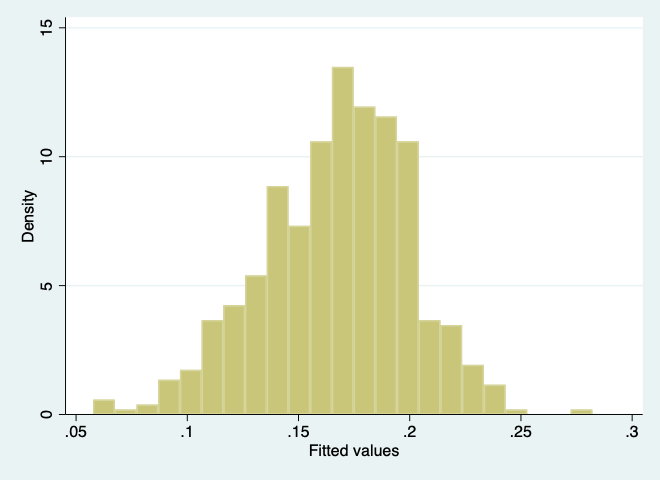
\includegraphics[scale =0.5]{p4_figure}
\end{center}

\bigskip

As seen in the histogram, all predicted probabilities are between zero and one.

\pagebreak

\subsection*{Problem 5 - Weighted Least Squares}

I tried running the baseline specification with using variance weighted least squares, but I get the following error: \textit{no groups with sufficient observations}. I suspect this error occurs because we do not have enough observation to compute the by-group variances to weight observations.  I am able to estimate a more parsimonious model using variance weighted least squares model by dropping religious/caste indicators, \texttt{muslim} and \texttt{Hindu\_SC\_Kat}, as well as \texttt{Client\_Married} due to multicollinearity.  Column (1) is the more parsimonious specification estimated using unweighted least squares and column (2) is that estimated using variance weighted least squares.

\bigskip

\begin{center}
\begin{tabular}{lcc} \hline
 & (1) & (2) \\
VARIABLES & taken\_new & taken\_new \\ \hline
 &  &  \\
Client\_Age & -4.51e-05 & -0.000535 \\
 & (0.00224) & (0.0198) \\
Client\_Education & -0.00325 & 0.00214 \\
 & (0.00400) & (0.0184) \\
HH\_Size & -0.0102 & 0.00353 \\
 & (0.00936) & (0.0576) \\
Treated & 0.0412 & -0.125 \\
 & (0.0332) & (0.373) \\
Constant & 0.216** & 0.490 \\
 & (0.107) & (0.877) \\
 &  &  \\
Observations & 532 & 65 \\
R-squared & 0.006 &  \\
 Weighted By & None & Variance \\ \hline
\multicolumn{3}{c}{ Robust standard errors in parentheses} \\
\multicolumn{3}{c}{ *** p$<$0.01, ** p$<$0.05, * p$<$0.1} \\
\end{tabular}

\end{center}

\bigskip

Coefficients in both regressions above are insignificant, which is consistent with the less parsimonious unweighted baseline linear probability estimates above.  Without weighting, the coefficients on \texttt{Client\_Education} and \texttt{HH\_Size} are larger compared to their variance weighted counterparts while the other coefficients are smaller.

\pagebreak

\subsection*{Problem 6 - Probit and Logit}

In the table below, there are estimates for the LPM with comma robust SEs (column 1), probit (column 2), and logit (column 3).

\bigskip

\begin{center}
\begin{tabular}{lccc} \hline
 & (1) & (2) & (3) \\
VARIABLES & taken\_new & taken\_new & taken\_new \\ \hline
 &  &  &  \\
Client\_Age & -2.83e-05 & 0.000154 & -0.000382 \\
 & (0.00227) & (0.00856) & (0.0157) \\
Client\_Married & 0.0117 & 0.0495 & 0.0931 \\
 & (0.0519) & (0.214) & (0.388) \\
Client\_Education & -0.00369 & -0.0146 & -0.0276 \\
 & (0.00410) & (0.0166) & (0.0300) \\
HH\_Size & -0.0113 & -0.0476 & -0.0854 \\
 & (0.00928) & (0.0379) & (0.0694) \\
HH\_Income & 3.14e-06 & 1.33e-05 & 2.23e-05 \\
 & (3.71e-06) & (1.44e-05) & (2.53e-05) \\
muslim & -0.00756 & -0.0326 & -0.0533 \\
 & (0.0365) & (0.147) & (0.263) \\
Hindu\_SC\_Kat & -0.0275 & -0.110 & -0.208 \\
 & (0.0510) & (0.215) & (0.395) \\
Treated & 0.0426 & 0.175 & 0.319 \\
 & (0.0335) & (0.142) & (0.259) \\
Constant & 0.199* & -0.853* & -1.374 \\
 & (0.117) & (0.459) & (0.835) \\
 &  &  &  \\
Observations & 532 & 532 & 532 \\
R-squared & 0.008 &  &  \\
 Model & LPM & Probit & Logit \\ \hline
\multicolumn{4}{c}{ Robust standard errors in parentheses} \\
\multicolumn{4}{c}{ *** p$<$0.01, ** p$<$0.05, * p$<$0.1} \\
\end{tabular}

\end{center}

\bigskip

The probit and the logit coefficients are not the same but they are similar, especially when comparing them to the LPM coefficients. These results make sense.  The probit uses the standard normal cdf as its link function, the logit uses its logistic function as the link function, and the LPM uses $f(x)=x$ as its link function.  The standard normal cdf and the logistic function are much closer to each than they are to $f(x)=x$.

\pagebreak

\subsection*{Problem 7 - Mean Partial Derivatives}

I compute the mean partial derivative for \texttt{Client\_Age} using six methods:

\begin{enumerate}
\item LPM coefficient.
\item \texttt{dprobit}
\item Analytically using a probit model. The mean partial derivative estimated as $\phi(x \beta') \beta_1$ where $\phi$ is the pdf of the standard normal.
\item Numerically using a probit model.  Estimate the probit model and predict the probability: $\hat{p}_i$.  Perturb \texttt{Client\_Age} by $\varepsilon = 0.01$ and reestimate the probit model to predict the probability: $\hat{p}^\varepsilon_i$. Compute the partial derivative for each observations: $\frac{\hat{p}_i - \hat{p}^\varepsilon_i}{\varepsilon}$. Compute the average across observations.
\item \texttt{Margins} for probit.
\item \texttt{Margins} for logit.
\end{enumerate}

\bigskip

\begin{center}
\begin{tabular}{ l l | r }
Model & Approach & Mean Partial Derivative Estimate\\ 
\hline
 LPM    & -                & -0.0000283 \\  
 Probit & \texttt{dprobit} &  0.0000382 \\
 Probit & Analytical       &  0.0000382 \\
 Probit & Numerical        &  0.0000386  \\
 Probit & \texttt{margins} &  0.0000382 \\
 Logit  & \texttt{margins} & -0.0000525
\end{tabular}
\end{center}

\bigskip

All the estimates are very close to zero, but some are positive and some are negative.  The differences between the mean partial derivative estimates partially boil down to how noisy the estimate of the coefficients on \texttt{Client\_Age} is.  In every regression (LPM, probit, and logit), the coefficient is statistically indistinguishable from zero.  Thus, the differences in the mean partial derivative estimates boil out to noise.  For the probit-based estimates, all but the numerical estimates are the same.  This must be due to \texttt{dprobit} and \texttt{margins} under the analytical derivative ``under the hood."

\pagebreak

\subsection*{Problem 8 - LPM with Quartic Age}

I add quadratic transformations of \texttt{Client\_Age} to the regression.  Column (1) is the baseline model and column (2) includes the additional terms.

\bigskip

\begin{center}
\begin{tabular}{lcc} \hline
 & (1) & (2) \\
VARIABLES & taken\_new & taken\_new \\ \hline
 &  &  \\
Client\_Age &  & -0.493*** \\
 &  & (0.168) \\
Client\_Age\_2 &  & 0.0199*** \\
 &  & (0.00621) \\
Client\_Age\_3 &  & -0.000336*** \\
 &  & (9.68e-05) \\
Client\_Age\_4 &  & 2.01e-06*** \\
 &  & (5.35e-07) \\
Client\_Married & 0.0117 & 0.0152 \\
 & (0.0518) & (0.0552) \\
Client\_Education & -0.00368 & -0.00315 \\
 & (0.00394) & (0.00411) \\
HH\_Size & -0.0113 & -0.00889 \\
 & (0.00927) & (0.00924) \\
HH\_Income & 3.14e-06 & 3.65e-06 \\
 & (3.71e-06) & (3.70e-06) \\
muslim & -0.00755 & -0.0128 \\
 & (0.0363) & (0.0361) \\
Hindu\_SC\_Kat & -0.0275 & -0.0333 \\
 & (0.0510) & (0.0507) \\
Treated & 0.0426 & 0.0465 \\
 & (0.0335) & (0.0334) \\
Constant & 0.198** & 4.518*** \\
 & (0.0779) & (1.605) \\
 &  &  \\
Observations & 532 & 532 \\
 R-squared & 0.008 & 0.031 \\ \hline
\multicolumn{3}{c}{ Robust standard errors in parentheses} \\
\multicolumn{3}{c}{ *** p$<$0.01, ** p$<$0.05, * p$<$0.1} \\
\end{tabular}

\end{center}

\bigskip

By their statistical significance, it appears that it is important to include these higher-order polynomial transformations of \texttt{Client\_Age}.  I numerically computing the mean partial derivative with respect to \texttt{Client\_Age} and get 2.32e-07.  So yes, adding the quadratic terms ``does better" in so much as the estimate is close to the probit model estimates.  However, there are now six observations with predicted probabilities outside the unit interval (five less than zero and one greater than one).

\begin{center}
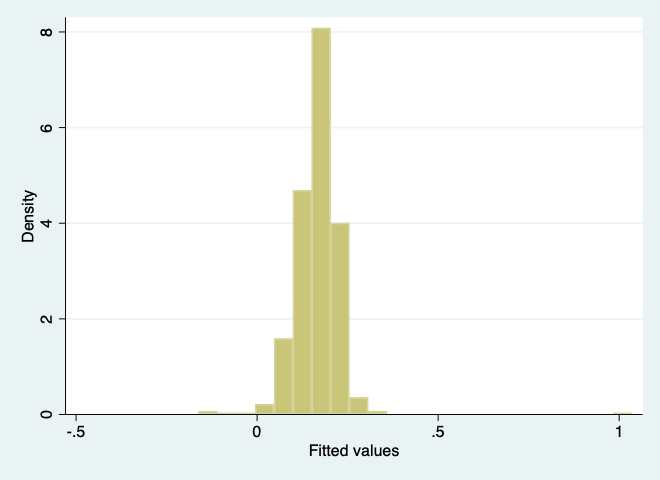
\includegraphics[scale =0.5]{p8_figure}
\end{center}

\subsection*{Problem 9 - LRI}

The log-likelihood of the baseline probit model is $\ln \hat{L} = -238.0747$ and the log-likelihood of a probit model with only a constant is $\ln L_0 = -240.2343$.  Thus, the LRI is $LRI = 1 - \frac{\ln \hat{L}}{\ln L_0} = 0.0090$. This matches the Stata output for pseudo-$R^2$. Since the LRI is low, this would suggest that the additional covariates do not explain more variation in outcome beyond what is captured by the constant.

\subsection*{Problem 10 - Correction Prediction Rates}

First, I consider correct prediction rates based on a 50 percent cutoff.  The idea behind the 50 percent cutoff is whether you're more likely to take out a loan than not. I get the following table:

\begin{center}
\begin{tabular}{ l | r r }
                   & $\hat{p} < 0.5$ & $\hat{p} > 0.5$\\ 
\hline
\texttt{taken\_new} = 1 &   0.8327 & 0.0 \\  
\texttt{taken\_new} = 0 & 0.1673   & 0.0 
\end{tabular}
\end{center}

This table is due to having none of the predicted probabilities are over 50 percent.  The correct prediction rate here is 0.41635 (i.e., 0.8327 times 50 percent). Second, I consider correct prediction rates based on a cutoff equal to unconditional probability of the outcome,  0.1673.  The idea behind this cutoff is whether you're more likely than a randomly selected person from the sample to take out a loan. I get the following table:

\begin{center}
\begin{tabular}{ l | r r }
 & $\hat{p} < 0.1673$ & $\hat{p} > 0.1673$\\ 
\hline
\texttt{taken\_new} = 1 & 0.4267 & 0.4060 \\  
\texttt{taken\_new} = 0 & 0.0602 & 0.1071
\end{tabular}
\end{center}

The correct prediction rate is now 0.2669 (i.e., 0.4267 times 50 percent plus 0.1071 times 50 percent).

\pagebreak

\subsection*{Problem 11 - In-Sample vs. Out-of-Sample Correct Prediction Rates}

My expectation is that in-sample correct prediction rates will be higher than out-of-sample correct prediction rates. First, based on a 50 percent cutoff, I get the following table for the estimation subsample:

\begin{center}
\begin{tabular}{ l | r r }
                   & $\hat{p} < 0.5$ & $\hat{p} > 0.5$\\ 
\hline
\texttt{taken\_new} = 1 &   0.8383 & 0.0 \\  
\texttt{taken\_new} = 0 & 0.1617   & 0.0 
\end{tabular}
\end{center}

Thus, the correct prediction rate is 0.4191. I get the following table for the non-estimation subsample:

\begin{center}
\begin{tabular}{ l | r r }
                   & $\hat{p} < 0.5$ & $\hat{p} > 0.5$\\ 
\hline
\texttt{taken\_new} = 1 &   0.8271 & 0.0 \\  
\texttt{taken\_new} = 0 & 0.1729   & 0.0 
\end{tabular}
\end{center}

Thus, the correct prediction rate is 0.4135. The higher correct prediction rate for the estimation sample has nothing to do with the accuracy of in-sample vs. out-of-sample prediction because all predicted values are less than 50 percent. The difference is only due to sample variation. Second, for a cutoff equal to unconditional probability of the outcome (0.1673), I get the following table for the estimation subsample:

\begin{center}
\begin{tabular}{ l | r r }
 & $\hat{p} < 0.1673$ & $\hat{p} > 0.1673$\\ 
\hline
\texttt{taken\_new} = 1 & 0.4812 & 0.3571 \\  
\texttt{taken\_new} = 0 & 0.0827 & 0.0789
\end{tabular}
\end{center}

Thus, the correct prediction rate is 0.2801. I get the following table for the non-estimation subsample:

\begin{center}
\begin{tabular}{ l | r r }
 & $\hat{p} < 0.1673$ & $\hat{p} > 0.1673$\\ 
\hline
\texttt{taken\_new} = 1 & 0.4436 & 0.3835 \\  
\texttt{taken\_new} = 0 & 0.1128 & 0.0602
\end{tabular}
\end{center}

Thus, the correct prediction rate is 0.2519.  This difference may be a confirmation that the prediction rate in-sample is better than out-of-sample. 

\pagebreak

\subsection*{Problem 12 - Interaction Term}

Below is the baseline probit model and the probit model with an interaction term for married and Muslim.

\bigskip

\begin{center}
\begin{tabular}{lcc} \hline
 & (1) & (2) \\
VARIABLES & taken\_new & taken\_new \\ \hline
 &  &  \\
Client\_Age & 0.000154 & 0.000931 \\
 & (0.00856) & (0.00868) \\
Client\_Married & 0.0495 & 0.156 \\
 & (0.214) & (0.281) \\
Client\_Education & -0.0146 & -0.0154 \\
 & (0.0166) & (0.0167) \\
HH\_Size & -0.0476 & -0.0502 \\
 & (0.0379) & (0.0381) \\
HH\_Income & 1.33e-05 & 1.26e-05 \\
 & (1.44e-05) & (1.45e-05) \\
muslim & -0.0326 & 0.206 \\
 & (0.147) & (0.421) \\
Hindu\_SC\_Kat & -0.110 & -0.114 \\
 & (0.215) & (0.215) \\
Treated & 0.175 & 0.182 \\
 & (0.142) & (0.142) \\
married\_muslim &  & -0.271 \\
 &  & (0.448) \\
Constant & -0.853* & -0.959* \\
 & (0.459) & (0.494) \\
 &  &  \\
 Observations & 532 & 532 \\ \hline
\multicolumn{3}{c}{ Standard errors in parentheses} \\
\multicolumn{3}{c}{ *** p$<$0.01, ** p$<$0.05, * p$<$0.1} \\
\end{tabular}

\end{center}

\bigskip

\subsection*{Problem 13 - Interaction Term Finite Differences}

I compute the interaction effect both with and without the terms highlighted by Ai and Norton (2003).  For the interaction effect without these terms, I use \texttt{margin} which automatically computes finite differences given a binary independent variable. The estimate of this interaction effect is -0.06719.  To compute the interaction effect with the terms highlighted by Ai and Norton (2003), I compute the predicted index from the probit.  Then I subtract the coefficient for each three dummies (married, Muslim, and married $\times$ Muslim).  This index, $I_0$, corresponds to the predicted value conditional on being unmarried and not Muslim for all observations.  Then I create a three variables based on this index: $I_1$ adds in the coefficient on married, $I_2$ adds in the coefficient on Muslim, and $I_{12}$ adds in all three coefficients.  Then the interaction affect for each observation is $\Phi(I_{12}) - \Phi(I_1) - \Phi(I_2) + \Phi(I_0)$.  The average of these finite differences is -0.0657. So the Ai and Norton (2003) terms slightly attenuate the estimated interaction effect.

\subsection*{Problem 14 - Interaction Term Finite Differences Variance}

I compute the variance of the finite differences for the interaction effect to be 0.00008.  The small variance stems from all coefficient estimating being quite small.

\pagebreak

\subsection*{Problem 15 - Heteroskedasticity Test}

I compute the residuals from the baseline LPM, square them, and regress them on the usual covariates:

\bigskip

\begin{center}
\begin{tabular}{lc} \hline
 & (1) \\
VARIABLES & residuals\_p\_2 \\ \hline
 &  \\
Client\_Age & 0.000168 \\
 & (0.00142) \\
Client\_Married & 0.00774 \\
 & (0.0348) \\
Client\_Education & -0.00213 \\
 & (0.00271) \\
HH\_Size & -0.00786 \\
 & (0.00612) \\
HH\_Income & 2.51e-06 \\
 & (2.42e-06) \\
muslim & -0.00633 \\
 & (0.0241) \\
Hindu\_SC\_Kat & -0.0168 \\
 & (0.0346) \\
Treated & 0.0282 \\
 & (0.0228) \\
Constant & 0.150** \\
 & (0.0752) \\
 &  \\
Observations & 532 \\
 R-squared & 0.008 \\ \hline
\multicolumn{2}{c}{ Standard errors in parentheses} \\
\multicolumn{2}{c}{ *** p$<$0.01, ** p$<$0.05, * p$<$0.1} \\
\end{tabular}

\end{center}

\bigskip

All coefficients are insignificant except for the constant.  These results indicate that heteroskedasticity is not a concern.

\pagebreak

\subsection*{Problem 16 - Probit with Heteroskedasticity}

The probit model with heteroskedasticity of the error term as a function of \texttt{Client\_Age} and \texttt{Client\_Education} is below.

\bigskip

\begin{center}
\begin{tabular}{lcc} \hline
 & (1) & (2) \\
VARIABLES & taken\_new & lnsigma \\ \hline
 &  &  \\
Client\_Age & -0.112 & 0.0285 \\
 & (0.137) & (0.0196) \\
Client\_Married & 0.129 &  \\
 & (0.846) &  \\
Client\_Education & -0.311 & 0.0694 \\
 & (0.256) & (0.0474) \\
HH\_Size & -0.226 &  \\
 & (0.197) &  \\
HH\_Income & 6.93e-05 &  \\
 & (7.23e-05) &  \\
muslim & -0.179 &  \\
 & (0.584) &  \\
Hindu\_SC\_Kat & -0.344 &  \\
 & (0.962) &  \\
Treated & 0.915 &  \\
 & (0.787) &  \\
Constant & 1.715 &  \\
 & (3.573) &  \\
 &  &  \\
 Observations & 532 & 532 \\ \hline
\multicolumn{3}{c}{ Standard errors in parentheses} \\
\multicolumn{3}{c}{ *** p$<$0.01, ** p$<$0.05, * p$<$0.1} \\
\end{tabular}

\end{center}

\bigskip

The critical value for the likelihood ratio test of \texttt{lnsigma=0} is 2.97 and it is distributed chi-squared with 2 degrees of freedom.  The resulting p-value is 0.2267, so we fail to reject the null of homoskedasticity.  This result confirms the finding in problem 15 of a lack of heteroskedasticity.

\pagebreak

\begin{landscape}

\section{Stata Log File}

\verbatiminput{analysis.log}

\end{landscape}

\end{document}

